\section{Application Acceleration}
\label{sec:acceleration}

\begin{figure*}[ht]
\centering
\vspace{0pt}
\begin{minipage}[c]{.3\textwidth}
	\includegraphics[width=0.27\paperwidth]{graphs/obj/hammingfull-crop.pdf}
	\caption{Nearest Neighbor with FlashBoost up to Two Nodes}
	\label{fig:result_hammingfull}
\end{minipage}\hfill
\vspace{0pt}
\begin{minipage}[c]{.3\textwidth}
	\includegraphics[width=0.27\paperwidth]{graphs/obj/hamming-crop.pdf}
	\caption{Nearest Neighbor with Single-Node Throttled FlashBoost}
	\label{fig:result_hamming}
\end{minipage}\hfill
\vspace{0pt}
\begin{minipage}[c]{.3\textwidth}
	\includegraphics[width=0.27\paperwidth]{graphs/obj/graph-crop.pdf}
	\caption{Graph Traversal Performance}
	\label{fig:result_graph}
\end{minipage}
\end{figure*}

In this section, we demonstrate the performance and benefits of the FlashBoost
architecture by presenting some accelerator demonstrations. 

\subsection{Nearest Neighbor Search}
\subsubsection{Description of Nearest Neighbor Search}

Nearest neighbor search is a classical problem with many applications. One of
the modern achievements in this field is Locality Sensitive Hashing~\cite{lsh}.
LSH hashes the dataset using multiple hash functions, so that
similar data is statistically likely to be hashed to similar buckets. When
querying, the query is hashed using the same hash functions, and only the data
in the matching buckets are actually compared. The bulk of the work during a
query process is traversing hash buckets and reading the corresponding data to
perform distance calculation. Because data pointed to by the hash buckets are
most likely scattered across the dataset, access patterns are quite random.

We have built a LSH query accelerator, where all of the data is stored in flash
and the distance calculation is done by the in-storage processor on the storage
device. For simplicity, we assume 8KB data items, and calculate the hamming
distance between the query data and each of the items in the hash bucket. The
software sends a stream of addresses from a hash bucket along with the query
data, and the system will return the index of the item most closely matching the
query. 

%By offloading computation to the in-storage accelerator, we
%show an order of magnitude performance improvement over the non-accelerated
%implementation. This puts our LSH implementation on par with a system where a
%request has a very high chance of being serviced by DRAM.

\subsubsection{Evaluation of Nearest Neighbor Search}

Figure~\ref{fig:result_hammingfull} shows the performance of a FlashBoost node
with an in-store processor against a DRAM-based machine running the same
workload. Compared to a DRAM implementation. FlashBoost has enough internal
bandwidth in the storage device that a single node of FlashBoost
outperforms DRAM up to 4 threads. It would require two FlashBoost nodes to match
the prformance of one 16-core RAM-based machine.

In order to demonstrate the benefits of the architecture, we show another
experiment where a FlashBoost node was bandwidth-throttled to the level of
commodity flash storage devices. FlashBoost was throttled to 600MB/s, which is
the bandwidth of the SATA 3.0 specification.
Figure~\ref{fig:result_hamming} shows the performance of nearest-neighbor search
with various data sources, normalized to the in-storage processing performance.
We compared FlashBoost against a high-cost fully DRAM configuration, as well as
realistic systems where some data cannot fit in DRAM.
Table~\ref{tab:nearest_neighbor} describes the benchmarks depicted in
Figure~\ref{fig:result_hamming}.

\begin{table}[h]\footnotesize
\begin{tabular}{l | p{0.25\paperwidth}}
\arraystretch{0.9}
Name & Description \\
\hline \hline
DRAM & Store all data in DRAM \\
ISP & Process data in in-storage accelerator \\
FlashBoost+SW & Use FlashBoost as raw storage \\
Seq Flash & All requests are sequential flash accesses \\
10\% Flash & Store most data in DRAM. 10\% chance of hitting flash \\
5\% Disk & Store most data in DRAM. 5\% chance of hitting disk \\
Full Flash & All requests go to flash \\
\hline
\end{tabular}
\caption{Nearest Neighbor Search Benchmarks}
\label{tab:nearest_neighbor}
\end{table}

It can be seen that streaming data directly from DRAM is obviously the fastest,
and scales linearly with thread count because with DRAM bandwidth, it becomes a
computation-bound workload. The configuration that uses an in-storage processor
to offload computation is consistently faster than the software implementation,
because there is no software overhead involved, and the in-storage processor can
process the data at wire speed. Since sequential flash access with two threads
outperforms FlashBoost, it can be seen that this performance difference is not
because of the flash device performance but because of architectural differences
and better optimized software. The reason random access into commodity flash
compared to sequential access show such performance is mosty likely because it
was optimized for a non-random access pattern. FlashBoost does not have this
problem. Compared to a fully flash-based execution, FlashBoost performs an order
of magnitude faster.

Using the full bandwidth of the storage system would
have made this gap even more pronounced, as the software's bandwidth would be
limited by the PCIe running at 1.6GB/s. It can be seen that when even most of
the data can fit in DRAM, even rare access into storage can have a significant
impact on performance. These results further reinforces our claim that better
storage systems are required for effective analytics of very large datasets.


\subsection{Graph Traversal}

\subsubsection{Description of Graph Traversal}

Efficient graph traversal is a very important component of any graph processing
system. Fast graph traversal enable solving many problems in graph theory,
including maximum flow, shortest path and graph search. It is also a very
latency-bound problem because one often cannot predict the next node to visit,
until the previous node is visited and processed. We demonstrate the performance
benefits of our FlashBoost architecture by implementing distributed graph
traversal that takes advantages of the in-storage processor and the integrated
storage network, which allows extremely low-latency access into both local and
remote flash storage.  

\subsubsection{Evaluation of Graph Traversal}

Figure~\ref{fig:result_graph} shows the performance of distributed graph traversal in
different configurations, normalized against the graph traversal
accelerator. Table~\ref{tab:graph} describes the benchmarks depitcted in
Figure~\ref{fig:result_graph}. Data was either read from distributed flash,
distributed DRAM, or a mixture of both. All experiments were made using the same
inter-controller network either as the integrated storage network or as a
separate network interface. This is for the sake of fair comparison because  the
inter-controller network has much better performance than Ethernet.

\begin{table}[h]\footnotesize
\begin{tabular}{l | p{0.25\paperwidth}}
\arraystretch{0.9}
Name & Description \\
\hline \hline
ISP & In-store processor requests data from remote storage over integrated network \\
SW & Software requests data from remote storage over integrated network \\
Flash & Software requests data from remote software to read from flash \\
50\% & Store requests data from remote software. 50\% chance of hitting flash \\
70\% & Store requests data from remote software. 30\% chance of hitting flash \\
DRAM & Software requests data from remote software. Data read from DRAM \\
\hline
\end{tabular}
\caption{Graph Traversal Benchmarks}
\label{tab:graph}
\end{table}

The performance difference between \emph{SW} and \emph{Flash} illustrates the
benefits of using the integrated network to reduce a layer of software access.
Performance of \emph{ISP} shows the benefits of reducing more software overhead
by having the ISP manage the graph traversal logic. 
The graph traversal accelerator can be seen to have nearly 3x
performance improvement compared to a naive implementation that uses flash only
as a storage device, and on par with a more expensive system where 70\% of the requests are
serviced by the DRAM.

%The difference latency has on graph traversal queries can
%be seen in Figure~\ref{fig:graph_accel}.
%\begin{figure}[ht!]
%	\centering
%
%		\hfill
%	\subfloat[Using ISP and Integrated Network]
%		{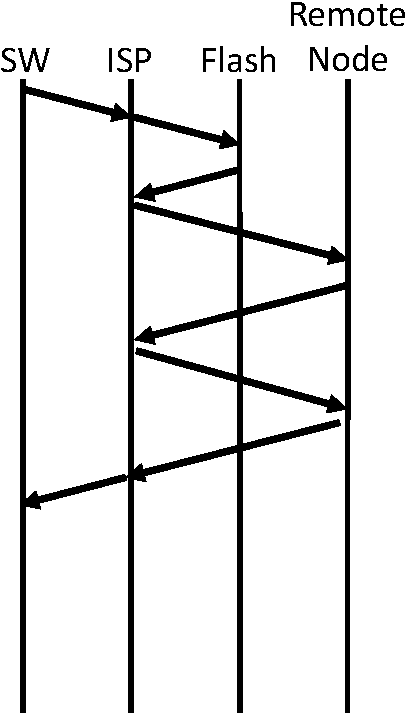
\includegraphics[width=0.12\textwidth]{figures/graph_isp-crop.pdf}}
%		\hfill
%	\subfloat[Using Software]
%		{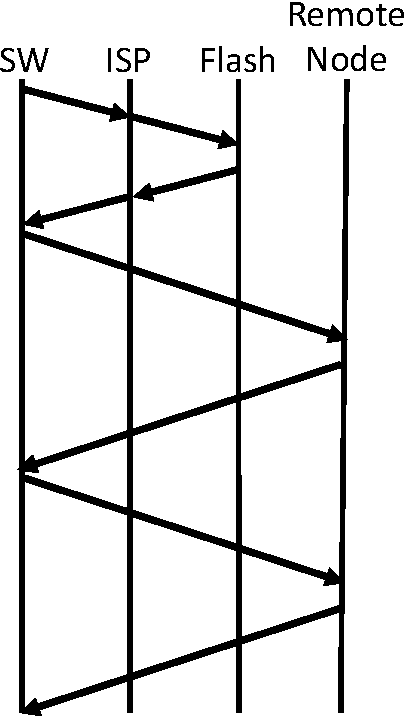
\includegraphics[width=0.12\textwidth]{figures/graph_sw-crop.pdf}}
%		\hfill
%	\caption{Graph Traversal Comparison}
%	\label{fig:graph_accel}
%\end{figure}

\subsection{String Search}

\subsubsection{Description of String Search}

String search is common operation in analytics, often used in
database table scans, DNA sequence matching and cheminformatics. It is 
primarily a sequential read and compare workload. We
examine its performance on FlashBoost with assistance from in-store Morris-Pratt (MP) 
string search engines~\cite{mpalgo} fully integrated with the file system, flash controller
and application software.  The software portion of string search initially sets
up the accelerator by transferring the target string pattern (needle) and a set
of precomputed MP constants over DMA. Then it consults the file system for a
list of physical addresses of the files to search (haystack).  This list is
streamed to the accelerator, which uses these addresses to request for pages
from the flash controller.  The accelerated MP engines may operate in parallel
either by searching multiple files or by dividing up the haystack into equal
segments (with some overlaps). This choice depends on the number of files and
size of each file. Since 4 read commands can saturate a single flash bus, we
use 4 engines per bus to maximize the flash bandwidth. Only
search results are returned to the server. 

\begin{figure}[t]
	\centering
	\includegraphics[width=0.35\textwidth]{graphs/obj/strstr-crop.pdf}
	\caption{String Search Bandwidth and CPU Utilization}
	\label{fig:result_strstr}
\end{figure}

\subsubsection{Evaluation of String Search}

We compared our implementation of hardware-accelerated string search running on
FlashBoost to the Linux Grep utility querying for exact string matches running
on both SSD and hard disk. Processing bandwidth and server CPU utilizations are
shown in Figure~\ref{fig:result_strstr}. We observe that the parallel MP
engines in FlashBoost are able to process a search at 1.1GB/s, which is 92\% of
the maximum sequential bandwidth a single flash board. Using FlashBoost, the
query consumes almost no CPU cycles on the host server since the query is
entirely offloaded and only the location of matched strings are returned, which
we assume is a tiny fraction of the file (0.01\% is used in our experiments).
This is 7.5x faster than software string search (Grep) on hard disks, which is
I/O bound by disk bandwidth and consumes 13\% CPU. On SSD, software string
search remains I/O bound by the storage device, but CPU utilization increases
significantly to 65\% even for this type of simple streaming compare operation.
This high utilization is problematic because string search is often only a small portion 
of more complex analytic queries that can quickly become compute bound.  As we
have shown in the results, FlashBoost can effectively alleviate this by
offloading search to the in-store processor thereby freeing up the server CPU
for other tasks. 
 

